\chapter{Approximations de l'opérateur d'impédance}
\label{sec:chap2}
\minitoc
\newpage
\sectionstar{Introduction}
Nous avons vu les expressions du symbole de l'opérateur d'impédance pour diverses géométries. Nous allons maintenant présenter plusieurs approximations de cet opérateur, leur symbole ainsi que les limites de ces approximations dans certains cas particuliers.
\section{Approximation de l'opérateur d'impédance pour un plan infini par une condition d'impédance d'ordre élevée}

  \subsection{Expression de la condition d'impédance d'ordre élevée}

    On sait que le symbole \(\hat{\mZ}(k_x,k_y)\) s'écrit

    \begin{multline}
        \hat \mZ_m = -k_{3m}
        \left(ik_{3m}\tan\left(k_{3m}d_m\right)\mI - \hat \mZ_{m-1}\mC_m\right) \\
        \left(k_{3m}\mI - i\tan\left(k_{3m}d_m\right)\hat \mZ_{m-1}\mC_m\right)^{-1}
        \mC_m^{-1}
    \end{multline}

    où la matrice \(\mC_m\) est telle que
    \begin{align}
       \mC_m &= \frac{1}{k_m\eta_m}
        \begin{bmatrix}
            k_m^2 - k_y^2 & k_xk_y\\
            k_xk_y & k_m^2 - k_y^2
        \end{bmatrix}
    \end{align}

    Dans le cadre de cette thèse, nous nous intéressons à la condition d'impédance d'\cite{aubakirov_electromagnetic_2014} qui s'exprime en tout point de la surface extérieur de notre objet telle que

    \begin{align}
        \left(I + b_1 \LD{} -b_2 \LR \right)\vE_t = \left(a_0 I + a_1 \LD{} - a_2 \LR \right)(\vn \pvect \vH) & \forall x \in \Gamma
    \end{align}

    Nous la nommons CI3.

    Pour approcher le symbole \(\hat{\mZ}\) que l'on a défini dans l'espace de Fourier, il convient donc d'exprimer les opérateurs \(\LD, \LR\) dans cet espace.

    % Pour cela, nous utiliserons la relation de \cite[Corollary 2,p. ~154]){yosida_functional_1995}:

    Par définition, on a
    \begin{align}
      \LD \vE_t & = \vgrads{} \vdivs{} \vE_t
    \end{align}

    Or

    \begin{align}
      \vE_t(x,y,z) & = \int_\RR\int_\RR \hat{\vE_t}(k_x,k_y,z)e^{ik_xx + ik_yy}\dd{k_x}\dd{k_y}
    \end{align}


    donc

    \begin{align}
      \LD \vE_t
      & = \vgrads{} \vdivs{} \vE_t
      \\
      &=\vgrads{} \int_\RR\int_\RR \hat{\vE_t}(k_x,k_y,z) \cdot \vgrads{} e^{ik_xx + ik_yy}\dd{k_x}\dd{k_y}
      \\
      &=\int_\RR \int_\RR \vhesss{}\left(\left( e^{ik_xx + ik_yy} \right) \hat{\vE_t}\right)(k_x,k_y,z)\dd{k_x}\dd{k_y}
    \end{align}

    On définit \(\hat{\LD}\) l'opérateur matriciel tel que
    \begin{align}
      \LD \vE_t
      &= \int_\RR\int_\RR \hat{\LD} \hat{\vE_t}(k_x,k_y,z)\dd{k_x}\dd{k_y}
    \end{align}

    \begin{equation}
      \hat{\LD}(k_x,k_y) = -
      \begin{bmatrix}
        k_x^2 & k_x k_y
        \\
        k_x k_y & k_y^2
      \end{bmatrix}
    \end{equation}


    Par définition, on a
    \begin{align}
      \LR \vE_t & = \vrots{} \vrots{} \vE_t
    \end{align}

    donc

    \begin{align}
      \LR \vE_t
      & = \vrots{} \vrots{} \vE_t
      \\
      &=\vrots{} \int_\RR\int_\RR \vgrads{}\left(e^{ik_xx + ik_yy}\right) \pvect \hat{\vE_t}(k_x,k_y,z)\dd{k_x}\dd{k_y}
      \\
      &= \int_\RR \int_\RR \left(\vhesss - \vlapls\right) \left(\left(e^{ik_xx + ik_yy}\right) \hat{\vE_t}\right)(k_x,k_y,z)\dd{k_x}\dd{k_y}
      \\
    \end{align}

    On définit \(\hat{\LR}\) l'opérateur matriciel tel que
    \begin{align}
      \LR \vE_t
      &= \int_\RR\int_\RR \hat{\LR} \hat{\vE_t}(k_x,k_y,z)\dd{k_x}\dd{k_y}
    \end{align}

    \begin{equation}
      \hat{\LR}(k_x,k_y) =
      \begin{bmatrix}
        k_y^2 & -k_x k_y
        \\
        -k_x k_y & k_x^2
      \end{bmatrix}
    \end{equation}

    On peut donc définir \(\hat{\mZ}_{IBC}\) l’opérateur matriciel associé à la condition d'impédance.

    \begin{multline}
        \hat{\mZ}_{IBC}(k_x,k_y) = \left(I + b_1 \hat{\LD}(k_x,k_y) - b_2 \hat{\LR}(k_x,k_y) \right)^{-1}
        \\
        \left(a_0 I + a_1 \hat{\LD}(k_x,k_y) - a_2 \hat{\LR}(k_x,k_y)\right)
    \end{multline}

    Pour calculer les coefficients de la CIOE, il faut minimiser la distance entre le symbole \(\hat{\mZ}(k_x,k_y)\) et \(\hat{\mZ}_{IBC}(k_x,k_y)\) \footnote{La distance est la norme de Frobenius}. Évidemment, il existe une infinité de combinaisons pour un couple \((k_x,k_y)\). Nous avons choisis de nous donner un grand nombre de couples et de minimiser au sens des moindres carrés.

    Pour tenir compte d'une onde plane homogène, il faut que \(k_x^2 + k_y^2\) soit inférieur à \(k_0^2\); au delà, nous reproduisons des ondes évanescentes. Nous avons constaté que prendre \(k_x^2 + k_y^2\) inférieur à \(2k_0\) est suffisant pour prendre en compte des ondes guidées dans le cas des matériaux sans pertes.

  \subsection{Le cas spécial de la condition de Leontovich}

    La condition de Leontovich consiste à approcher le symbole par une constante, et donc d'avoir \(a_1=a_2=b_1=b_2=0\). Dans le paragraphe précèdent, cela revient à chercher la valeur moyenne du symbole. Cependant, cette condition rend compte de l'impédance à incidence normale. Dans ce cas particulier, nous ne réaliserons pas de minimisation mais on fixera cette constante à la valeur du symbole en \((0,0)\).

    \begin{equation}
      a_0 = \hat{\mZ}(0,0)
    \end{equation}

  \subsection{Résultats numériques}

      La figure \ref{fig:imp_fourier:plan:hoppe:33:hoibc} permet de vérifier les résultats de \cite[p.~33]{hoppe_impedance_1995} pour une couche de matériau sans perte où il n'y a pas de \(k_x\) réel tel que \(kd=\frac{\pi}{2} + n \pi\) donc pas d'asymptote pour le symbole. La condition d'impédance d'ordre élevé est bien meilleure que la condition de Leontovich.
      \begin{figure}[!hbt]
          \centering
          \tikzsetnextfilename{Z_HOPPE_33_plan_hoibc_TM}
\begin{tikzpicture}[scale=1]
  \begin{axis}[
          title={Polarisation TM},
          ylabel={\(\Im(\hat{Z}(k_x,0)\)},
          xlabel={\(k_x\slash k_0\)},
          width=0.4\textwidth,
          xmin=0,
          xmax=2,
          mark repeat=20,
          legend pos=outer north east
      ]
      \addplot [color=black,mark=square*] table [col sep=comma, x={s1}, y={Im(z_ex.tm)}] {csv/HOPPE_33/HOPPE_33.z_ex.P.csv};
      % \addlegendentry{Exact};

      \addplot [color=blue,mark=x] table [col sep=comma, x={s1}, y={Im(z_ibc0.tm)}] {csv/HOPPE_33/HOPPE_33.z_ibc.IBC_ibc0_TYPE_P_SUC_F.csv};
      % \addlegendentry{CI0};

      \addplot [color=red,mark=diamond*] table [col sep=comma, x={s1}, y={Im(z_ibc3.tm)}] {csv/HOPPE_33/HOPPE_33.z_ibc.IBC_ibc3_TYPE_P_SUC_F.csv};
      % \addlegendentry{CI3};
  \end{axis}
\end{tikzpicture}
\tikzsetnextfilename{Z_HOPPE_33_plan_hoibc_TE}
\begin{tikzpicture}[scale=1]
  \begin{axis}[
          title={Polarisation TE},
          ylabel={},
          xlabel={\(k_x\slash k_0\)},
          width=0.4\textwidth,
          xmin=0,
          xmax=2,
          mark repeat=20,
          legend pos=outer north east
      ]
      \addplot [color=black,mark=square*] table [col sep=comma, x={s1}, y={Im(z_ex.te)}] {csv/HOPPE_33/HOPPE_33.z_ex.P.csv};
      \addlegendentry{Exact};

      \addplot [color=blue,mark=x] table [col sep=comma, x={s1}, y={Im(z_ibc0.te)},color=] {csv/HOPPE_33/HOPPE_33.z_ibc.IBC_ibc0_TYPE_P_SUC_F.csv};
      \addlegendentry{CI0};

      \addplot [color=red,mark=diamond*] table [col sep=comma, x={s1}, y={Im(z_ibc3.te)}] {csv/HOPPE_33/HOPPE_33.z_ibc.IBC_ibc3_TYPE_P_SUC_F.csv};
      \addlegendentry{CI3};
  \end{axis}
\end{tikzpicture}
          \caption[CIOE sur empilement de Hoppe & Rahmat-Samii p.~33]{\(\eps = 4, \mu = 1, d=0.015\text{m}, f=1\text{GHz}\)}
          \label{fig:imp_fourier:plan:hoppe:33:hoibc}
      \end{figure}
      \begin{table}[!hbt]
        \centering
        % On fait deux tables de même hauteur
        \begin{coefftable}{\hyperlink{ci0}{CI0}}
          a_0 & \NaN + \NaN i
          \\
          \\
          \\
          \\
          \\
        \end{coefftable}
        \begin{coefftable}{\hyperlink{ci3}{CI3}}
          a_0 & \NaN + \NaN i
          \\
          a_1 & \NaN + \NaN i
          \\
          a_2 & \NaN + \NaN i
          \\
          b_1 & \NaN + \NaN i
          \\
          b_2 & \NaN + \NaN i
        \end{coefftable}
        \caption{Coefficients associés à la figure \ref{fig:imp_fourier:plan:hoppe:33:hoibc}}
        \label{tab:imp_fourier:plan:hoppe:33:hoibc}
      \end{table}

      La figure \ref{fig:imp_fourier:plan:soudais:hoibc} permet de vérifier les résultats de \cite[p.~11]{soudais_3d_2017} pour une couche de matériau sans perte où il y a une asymptote pour le symbole. La condition d'impédance d'ordre élevé capture cet asymptote grâce à son numérateur et est donc bien meilleure que la condition de Leontovich.
      \begin{figure}[!hbt]
          \centering
          \begin{tikzpicture}[scale=1]
    \begin{axis}[
            title={Polarisation TM},
            ylabel={\(\Im(\hat{Z}(k_x,0)\)},
            xlabel={\(k_x\slash k_0\)},
            width=0.4\textwidth,
            xmin=0,
            xmax=1.8,
            ymin=-1E+1,
            ymax=1E+1,
            restrict y to domain=-30:30,
            mark repeat=40,
            legend pos=outer north east
        ]
        \addplot [color=black,mark=square*] table [col sep=comma, x={s1}, y={Im(z_ex.tm)}] {csv/ICEAA_11/ICEAA_11.z_ex.P.csv};
        % \addlegendentry{Exact};

        \addplot [color=blue,mark=x] table [col sep=comma, x={s1}, y={Im(z_ibc0.tm)}] {csv/ICEAA_11/ICEAA_11.z_ibc.IBC_ibc0_TYPE_P_SUC_F.csv};
        % \addlegendentry{CI0};

        \addplot [color=red,mark=diamond*] table [col sep=comma, x={s1}, y={Im(z_ibc3.tm)}] {csv/ICEAA_11/ICEAA_11.z_ibc.IBC_ibc3_TYPE_P_SUC_F.csv};
        % \addlegendentry{CI3};
    \end{axis}
\end{tikzpicture}
\begin{tikzpicture}[scale=1]
    \begin{axis}[
            title={Polarisation TE},
            ylabel={},
            xlabel={\(k_x\slash k_0\)},
            width=0.4\textwidth,
            xmin=0,
            xmax=1.8,
            ymin=-1E+1,
            ymax=1E+1,
            restrict y to domain=-30:30,
            mark repeat=40,
            legend pos=outer north east
        ]
        \addplot [color=black,mark=square*] table [col sep=comma, x={s1}, y={Im(z_ex.te)}] {csv/ICEAA_11/ICEAA_11.z_ex.P.csv};
        \addlegendentry{Exact};

        \addplot [color=blue,mark=x] table [col sep=comma, x={s1}, y={Im(z_ibc0.te)},color=] {csv/ICEAA_11/ICEAA_11.z_ibc.IBC_ibc0_TYPE_P_SUC_F.csv};
        \addlegendentry{CI0};

        \addplot [color=red,mark=diamond*] table [col sep=comma, x={s1}, y={Im(z_ibc3.te)}] {csv/ICEAA_11/ICEAA_11.z_ibc.IBC_ibc3_TYPE_P_SUC_F.csv};
        \addlegendentry{CI3};
    \end{axis}
\end{tikzpicture}
          \caption[CIOE sur empilement de P.~Soudais p.~11]{Partie imaginaire des coefficients diagonaux de \(\hat\mZ\) pour \(\eps = 4, \mu = 1, d=0.035\text{m}, f=12\text{GHz}\)}
          \label{fig:imp_fourier:plan:soudais:hoibc}
      \end{figure}
      \begin{table}[!hbt]
        \centering
        % On fait deux tables de même hauteur
        \begin{coefftable}{\hyperlink{ci0}{CI0}}
          a_0 & \NaN + \NaN i
          \\
          \\
          \\
          \\
          \\
        \end{coefftable}
        \begin{coefftable}{\hyperlink{ci3}{CI3}}
          a_0 & \NaN + \NaN i
          \\
          a_1 & \NaN + \NaN i
          \\
          a_2 & \NaN + \NaN i
          \\
          b_1 & \NaN + \NaN i
          \\
          b_2 & \NaN + \NaN i
        \end{coefftable}
        \caption{Coefficients associés à la figure \ref{fig:imp_fourier:plan:soudais:hoibc}}
        \label{tab:imp_fourier:plan:soudais:hoibc}
      \end{table}

      On voit sur la figure \ref{fig:reflex_fourier:plan:soudais:hoibc} que cela va de même pour la matrice de réflexion. On déjà vu sur le symbole exact l'onde guidée qui fait diverger ce coefficient de réflexion TM, et on remarque que la CI3 la reproduit assez fidèlement.
      \begin{figure}[!hbt]
          \centering
                    \begin{tikzpicture}[scale=1]
              \begin{axis}[
                      title={Polarisation TM},
                      ylabel={\(|\hat{R}(k_x,0)|\)},
                      xlabel={\(k_x\slash k_0\)},
                      width=0.4\textwidth,
                      ymin=0,
                      ymax=+3E+01,
                      restrict y to domain=0:+4E+01,
                      xmin=0,
                      xmax=1.8,
                      mark repeat=40,
                      legend pos=outer north east
                  ]
                  \addplot [color=black,mark=square*] table [col sep=comma, x={s1}, y={Abs(r_ex.tm)}] {csv/ICEAA_11/ICEAA_11.r_ex.P.csv};
                  % \addlegendentry{Exact};

                  \addplot [color=blue,mark=x] table [col sep=comma, x={s1}, y={Abs(r_ibc0.tm)}] {csv/ICEAA_11/ICEAA_11.r_ibc.IBC_ibc0_TYPE_P_SUC_F.csv};
                  % \addlegendentry{CI0};

                  \addplot [color=red,mark=diamond*] table [col sep=comma, x={s1}, y={Abs(r_ibc3.tm)}] {csv/ICEAA_11/ICEAA_11.r_ibc.IBC_ibc3_TYPE_P_SUC_F.csv};
                  % \addlegendentry{CI3};
              \end{axis}
          \end{tikzpicture}
          \begin{tikzpicture}[scale=1]
              \begin{axis}[
                      title={Polarisation TE},
                      ylabel={},
                      xlabel={\(k_x\slash k_0\)},
                      width=0.4\textwidth,
                      xmin=0,
                      xmax=1.8,
                      ymin=0,
                      ymax=+3E+01,
                      mark repeat=40,
                      legend pos=outer north east
                  ]
                  \addplot [color=black,mark=square*] table [col sep=comma, x={s1}, y={Abs(r_ex.te)}] {csv/ICEAA_11/ICEAA_11.r_ex.P.csv};
                  \addlegendentry{Exact};

                  \addplot [color=blue,mark=x] table [col sep=comma, x={s1}, y={Abs(r_ibc0.te)},color=] {csv/ICEAA_11/ICEAA_11.r_ibc.IBC_ibc0_TYPE_P_SUC_F.csv};
                  \addlegendentry{CI0};

                  \addplot [color=red,mark=diamond*] table [col sep=comma, x={s1}, y={Abs(r_ibc3.te)}] {csv/ICEAA_11/ICEAA_11.r_ibc.IBC_ibc3_TYPE_P_SUC_F.csv};
                  \addlegendentry{CI3};
              \end{axis}
          \end{tikzpicture}
          \caption[CIOE sur empilement de P.~Soudais p.~11]{Module des coefficients diagonaux de \(\mR\) pour \(\eps = 4, \mu = 1, d=0.035\text{m}, f=12\text{GHz}\)}
          \label{fig:reflex_fourier:plan:soudais:hoibc}
      \end{figure}

      La figure \ref{fig:imp_fourier:plan:triple_asymptote:hoibc} montre la limite de la CI3 pour capturer 3 asymptotes. Pour cela, il faudrait utiliser une CI d'ordre au moins 6.

      L'expression de cette CIOE que l'on nomme \hyperlink{ci7}{CI7} est
      \begin{equation}
        \left(\oI + \sum_{i=1}^3 \left(d_{i} \frac{\LD^i}{k_0^2} + e_{i} \frac{(-\LR)^i}{k_0^2} \right)\right)\vE_t = \left(a_0 \oI + \sum_{i=1}^3 \left(b_{i} \frac{\LD^i}{k_0^2} + c_{i} \frac{(-\LR)^i}{k_0^2} \right)\right)\vJ
      \end{equation}

      \begin{figure}[!hbt]
          \centering
          \tikzsetnextfilename{Z_triple_asymptote_plan_hoibc.TM}
\begin{tikzpicture}[scale=1]
    \begin{axis}[
            title={Polarisation TM},
            ylabel={\(\Im(\hat{Z}(k_x,0)\)},
            xlabel={\(k_x\slash k_0\)},
            width=0.4\textwidth,
            xmin=0,
            xmax=1.999,
            ymin=-10,
            ymax=10,
            restrict y to domain=-300:300,
            mark repeat=200,
            legend pos=outer north east
        ]
        \addplot [color=black,mark=square*] table [col sep=comma, x={s1}, y={Im(z_ex.tm)}] {csv/triple_asymptote/triple_asymptote.z_ex.MODE_2_TYPE_P.csv};
        % \addlegendentry{Exact};

        \addplot [color=blue,mark=x] table [col sep=comma, x={s1}, y={Im(z_ibc0.tm)}] {csv/triple_asymptote/triple_asymptote.z_ibc.IBC_ibc0_SUC_F_MODE_2_TYPE_P.csv};
        % \addlegendentry{CI0};

        \addplot [color=red,mark=diamond*] table [col sep=comma, x={s1}, y={Im(z_ibc3.tm)}] {csv/triple_asymptote/triple_asymptote.z_ibc.IBC_ibc3_SUC_F_MODE_2_TYPE_P.csv};
        % \addlegendentry{CI3};

        \addplot [color=cyan,mark=pentagon*] table [col sep=comma, x={s1}, y={Im(z_ibc7.tm)}] {csv/triple_asymptote/triple_asymptote.z_ibc.IBC_ibc7_SUC_F_MODE_2_TYPE_P.csv};
        % \addlegendentry{CI7};
    \end{axis}
\end{tikzpicture}
\tikzsetnextfilename{Z_triple_asymptote_plan_hoibc.TE}
\begin{tikzpicture}[scale=1]
    \begin{axis}[
            title={Polarisation TE},
            ylabel={},
            xlabel={\(k_x\slash k_0\)},
            width=0.4\textwidth,
            xmin=0,
            xmax=1.999,
            ymin=-10,
            ymax=10,
            restrict y to domain=-300:300,
            mark repeat=200,
            legend pos=outer north east
        ]
        \addplot [color=black,mark=square*] table [col sep=comma, x={s1}, y={Im(z_ex.te)}] {csv/triple_asymptote/triple_asymptote.z_ex.MODE_2_TYPE_P.csv};
        \addlegendentry{Exact};

        \addplot [color=blue,mark=x] table [col sep=comma, x={s1}, y={Im(z_ibc0.te)}] {csv/triple_asymptote/triple_asymptote.z_ibc.IBC_ibc0_SUC_F_MODE_2_TYPE_P.csv};
        \addlegendentry{CI0};

        \addplot [color=red,mark=diamond*] table [col sep=comma, x={s1}, y={Im(z_ibc3.te)}] {csv/triple_asymptote/triple_asymptote.z_ibc.IBC_ibc3_SUC_F_MODE_2_TYPE_P.csv};
        \addlegendentry{CI3};

        \addplot [color=cyan,mark=pentagon*] table [col sep=comma, x={s1}, y={Im(z_ibc7.te)}] {csv/triple_asymptote/triple_asymptote.z_ibc.IBC_ibc7_SUC_F_MODE_2_TYPE_P.csv};
        \addlegendentry{CI7};                  
    \end{axis}
\end{tikzpicture}
          \caption[CIOE sur empilement avec triple asymptote]{Partie imaginaire des coefficients diagonaux de \(\mZ\) pour \(\eps = 4, \mu = 1, d=0.2\text{m}, f=1\text{GHz}\)}
          \label{fig:imp_fourier:plan:triple_asymptote:hoibc}
      \end{figure}
      \begin{table}[!hbt]
        \centering
        % On fait deux tables de même hauteur
        \begin{coefftable}{\hyperlink{ci0}{CI0}}
          a_0 & \NaN + \NaN i
          \\
          \\
          \\
          \\
          \\
          \\
          \\
          \\
          \\
          \\
          \\
          \\
          \\
        \end{coefftable}
        \begin{coefftable}{\hyperlink{ci3}{CI3}}
          a_0 & \NaN + \NaN i
          \\
          a_1 & \NaN + \NaN i
          \\
          a_2 & \NaN + \NaN i
          \\
          b_1 & \NaN + \NaN i
          \\
          b_2 & \NaN + \NaN i
          \\
          \\
          \\
          \\
          \\
          \\
          \\
          \\
          \\
        \end{coefftable}
        \begin{coefftable}{\hyperlink{ci7}{CI7}}
          a_0 & \NaN + \NaN i
          \\
          b_1 & \NaN + \NaN i
          \\
          c_1 & \NaN + \NaN i
          \\
          d_1 & \NaN + \NaN i
          \\
          e_1 & \NaN + \NaN i
          \\
          b_2 & \NaN + \NaN i
          \\
          c_2 & \NaN + \NaN i
          \\
          d_2 & \NaN + \NaN i
          \\
          e_2 & \NaN + \NaN i
          \\
          b_3 & \NaN + \NaN i
          \\
          c_3 & \NaN + \NaN i
          \\
          e_3 & \NaN + \NaN i
          \\
          e_3 & \NaN + \NaN i
        \end{coefftable}
        \caption{Coefficients associés à la figure \ref{fig:imp_fourier:plan:triple_asymptote:hoibc}}
        \label{tab:imp_fourier:plan:triple_asymptote:hoibc}
      \end{table}
      Il faut donc une CIOE d'ordre 2 fois le nombre d'asymptote que l'on rencontre sur notre balayage.


  \subsection{Lien avec les CIOE de \cite{stupfel_implementation_2015}}

    Dans cet article sont introduites les CIOE
    \begin{itemize}
      \item CI01
        \begin{equation}
          \vE_t = \left(a_0\oI + a_1\LL\right)\vJ
        \end{equation}
      \item CI1
        \begin{equation}
          \left(\oI + b\LL \right)\vE_t = \left(a_0\oI + a_1\LL\right)\vJ
        \end{equation}
    \end{itemize}

    L'opérateur \(\LL\) est le laplacien tangentiel \(\lapls\) appliqué à chaque composante. Le multiplicateur de Fourier associé est la matrice
    \begin{equation}
      \hat{\mL}  = -
      \begin{bmatrix}
        k_x^2 + k_y^2 & 0
        \\
        0 & k_x^2 + k_y^2
      \end{bmatrix}
    \end{equation}

    Le multiplicateur est multiple de l'identité ce qui en fait un mauvais candidat convenu de la nature diagonale mais non multiple de l’identité du symbole. La figure \ref{fig:imp_fourier:plan:stupfel:hoibc} présente donc quelques résultats où l'on voit bien la limite de ces CIOE.
    \begin{figure}[!hbt]
      \centering
      \begin{tikzpicture}[scale=1]
    \begin{axis}[
            title={Polarisation TM},
            ylabel={\(|\hat{Z}(k_x,0)|\)},
            xlabel={\(k_x\slash k_0\)},
            width=0.4\textwidth,
            xmin=0,
            xmax=1.5,
            ymin=0.15,
            ymax=0.25,
            restrict y to domain=0:11,
            mark repeat=10,
            legend pos=outer north east
        ]
        \addplot [color=black,mark=square*] table [col sep=comma, x={s1}, y={Abs(z_ex.tm)}] {csv/M1/M1.z_ex.P.csv};

        \addplot [color=blue,mark=x] table [col sep=comma, x={s1}, y={Abs(z_ibc0.tm)}] {csv/M1/M1.z_ibc.IBC_ibc0_TYPE_P_SUC_F.csv};

        \addplot [color=green!50!black,mark=pentagon*] table [col sep=comma, x={s1}, y={Abs(z_ibc01.tm)}] {csv/M1/M1.z_ibc.IBC_ibc01_TYPE_P_SUC_F.csv};

        \addplot [color=orange,mark=*] table [col sep=comma, x={s1}, y={Abs(z_ibc1.tm)}] {csv/M1/M1.z_ibc.IBC_ibc1_TYPE_P_SUC_F.csv};

        \addplot [color=red,mark=diamond*] table [col sep=comma, x={s1}, y={Abs(z_ibc3.tm)}] {csv/M1/M1.z_ibc.IBC_ibc3_TYPE_P_SUC_F.csv};
    \end{axis}
\end{tikzpicture}
\begin{tikzpicture}[scale=1]
    \begin{axis}[
            title={Polarisation TE},
            ylabel={},
            xlabel={\(k_x\slash k_0\)},
            width=0.4\textwidth,
            xmin=0,
            xmax=1.5,
            ymin=0.15,
            ymax=0.25,
            mark repeat=10,
            restrict y to domain=0:11,
            legend pos=outer north east
        ]
        \addplot [color=black,mark=square*] table [col sep=comma, x={s1}, y={Abs(z_ex.te)}] {csv/M1/M1.z_ex.P.csv};
        \addlegendentry{Exact};

        \addplot [color=blue,mark=x] table [col sep=comma, x={s1}, y={Abs(z_ibc0.te)},color=] {csv/M1/M1.z_ibc.IBC_ibc0_TYPE_P_SUC_F.csv};
        \addlegendentry{CI0};

        \addplot [color=green!50!black,mark=pentagon*] table [col sep=comma, x={s1}, y={Abs(z_ibc01.te)}] {csv/M1/M1.z_ibc.IBC_ibc01_TYPE_P_SUC_F.csv};
        \addlegendentry{CI01};

        \addplot [color=orange,mark=*] table [col sep=comma, x={s1}, y={Abs(z_ibc1.te)}] {csv/M1/M1.z_ibc.IBC_ibc1_TYPE_P_SUC_F.csv};
        \addlegendentry{CI1};

        \addplot [color=red,mark=diamond*] table [col sep=comma, x={s1}, y={Abs(z_ibc3.te)}] {csv/M1/M1.z_ibc.IBC_ibc3_TYPE_P_SUC_F.csv};
        \addlegendentry{CI3};

    \end{axis}
\end{tikzpicture}
      \caption[CIOE sur empilement de B.~Stupfel p.~1661]{Module des coefficients diagonaux de \(\hat\mZ\) pour \(\eps = 1-i, \mu = 1, d=0.05\text{m}, f=0.2\text{GHz}\)}
      \label{fig:imp_fourier:plan:stupfel:hoibc}
    \end{figure}
      \begin{table}[!hbt]
        \centering
        % On fait deux tables de même hauteur
        \begin{coefftable}{\hyperlink{ci0}{CI0}}
          a_0 & \NaN + \NaN i
          \\
          \\
        \end{coefftable}
        \begin{coefftable}{\hyperlink{ci01}{CI01}}
          a_0 & \NaN + \NaN i
          \\
          a_1 & \NaN + \NaN i
        \end{coefftable}

        \begin{coefftable}{\hyperlink{ci1}{CI1}}
          a_0 & \NaN + \NaN i
          \\
          a_1 & \NaN + \NaN i
          \\
          b  & \NaN + \NaN i
          \\
          \\
          \\
        \end{coefftable}
        \begin{coefftable}{\hyperlink{ci3}{CI3}}
          a_0 & \NaN + \NaN i
          \\
          a_1 & \NaN + \NaN i
          \\
          a_2 & \NaN + \NaN i
          \\
          b_1 & \NaN + \NaN i
          \\
          b_2 & \NaN + \NaN i
        \end{coefftable}
        \caption{Coefficients associés à la figure \ref{fig:imp_fourier:plan:stupfel:hoibc}}
        \label{tab:imp_fourier:plan:stupfel:hoibc}
      \end{table}
    \begin{figure}[!hbt]
      \centering
      \tikzsetnextfilename{R_cioe_2015_plan_hoibc_TM}
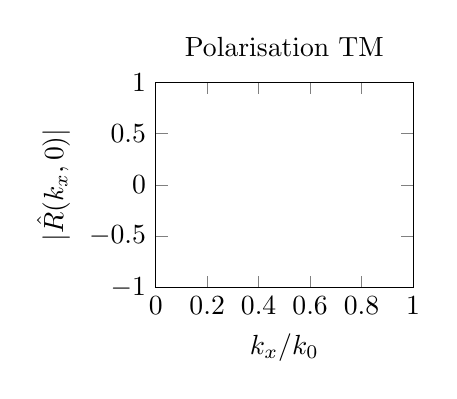
\begin{tikzpicture}[scale=1]
    \begin{axis}[
            title={Polarisation TM},
            ylabel={\(|\hat{R}(k_x,0)|\)},
            xlabel={\(k_x\slash k_0\)},
            width=0.4\textwidth,
            xmin=0,
            xmax=1,
            ymin=-1,
            ymax=1,
            mark repeat=15,
            legend pos=outer north east
        ]
        % \addplot [color=black,mark=square*] table [col sep=comma, x={s1}, y={Abs(r_ex.tm)}] {csv/STUPFEL/STUPFEL.r_ex.MODE_2_TYPE_P.csv};

        % \addplot [color=blue,mark=x] table [col sep=comma, x={s1}, y={Abs(r_ibc0.tm)}] {csv/STUPFEL/STUPFEL.r_ibc.IBC_ibc0_SUC_F_MODE_2_TYPE_P.csv};

        % \addplot [color=green!50!black,mark=pentagon*] table [col sep=comma, x={s1}, y={Abs(r_ibc01.tm)}] {csv/STUPFEL/STUPFEL.r_ibc.IBC_ibc01_SUC_F_MODE_2_TYPE_P.csv};

        % \addplot [color=orange,mark=*] table [col sep=comma, x={s1}, y={Abs(r_ibc1.tm)}] {csv/STUPFEL/STUPFEL.r_ibc.IBC_ibc1_SUC_F_MODE_2_TYPE_P.csv};

        % \addplot [color=red,mark=diamond*] table [col sep=comma, x={s1}, y={Abs(r_ibc3.tm)}] {csv/STUPFEL/STUPFEL.r_ibc.IBC_ibc3_SUC_F_MODE_2_TYPE_P.csv};
    \end{axis}
\end{tikzpicture}
\tikzsetnextfilename{R_cioe_2015_plan_hoibc_TE}
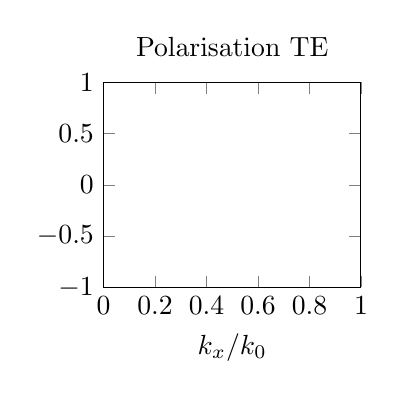
\begin{tikzpicture}[scale=1]
    \begin{axis}[
            title={Polarisation TE},
            ylabel={},
            xlabel={\(k_x\slash k_0\)},
            width=0.4\textwidth,
            xmin=0,
            xmax=1,
            ymin=-1,
            ymax=1,
            mark repeat=15,
            legend pos=outer north east
        ]
        % \addplot [color=black,mark=square*] table [col sep=comma, x={s1}, y={Abs(r_ex.te)}] {csv/STUPFEL/STUPFEL.r_ex.MODE_2_TYPE_P.csv};
        % \addlegendentry{Exact};

        % \addplot [color=blue,mark=x] table [col sep=comma, x={s1}, y={Abs(r_ibc0.te)},color=] {csv/STUPFEL/STUPFEL.r_ibc.IBC_ibc0_SUC_F_MODE_2_TYPE_P.csv};
        % \addlegendentry{CI0};

        % \addplot [color=green!50!black,mark=pentagon*] table [col sep=comma, x={s1}, y={Abs(r_ibc01.te)}] {csv/STUPFEL/STUPFEL.r_ibc.IBC_ibc01_SUC_F_MODE_2_TYPE_P.csv};
        % \addlegendentry{CI01};

        % \addplot [color=orange,mark=*] table [col sep=comma, x={s1}, y={Abs(r_ibc1.te)}] {csv/STUPFEL/STUPFEL.r_ibc.IBC_ibc1_SUC_F_MODE_2_TYPE_P.csv};
        % \addlegendentry{CI1};

        % \addplot [color=red,mark=diamond*] table [col sep=comma, x={s1}, y={Abs(r_ibc3.te)}] {csv/STUPFEL/STUPFEL.r_ibc.IBC_ibc3_SUC_F_MODE_2_TYPE_P.csv};
        % \addlegendentry{CI3};

    \end{axis}
\end{tikzpicture}
      \caption[CIOE sur empilement de B.~Stupfel p.~1661]{Module des coefficients diagonaux de \(\mR\) pour \(\eps = 1-i, \mu = 1, d=0.05\text{m}, f=0.2\text{GHz}\)}
      \label{fig:reflex_fourier:plan:stupfel:hoibc}
    \end{figure}
\section{Approximation de l'opérateur d'impédance pour un cylindre infini}

  \subsection{Expression de la condition d'impédance d'ordre élevée}

    On reprend les méthodes et résultats de la partie précédente.
    Soit \(R_{ext}\) le rayon de la couche extérieure.
    Le changement de système de coordonnées modifie l'expression des opérateurs \(\LD, \LR\).

    \begin{equation}
      \hat{\LD}(n,k_z) = -
      \begin{bmatrix}
        \left(\frac{n}{R_{ext}}\right)^2 & \frac{n}{R_{ext}} k_z
        \\
        \frac{n}{R_{ext}} k_z & k_z^2
      \end{bmatrix}
    \end{equation}

    \begin{equation}
      \hat{\LR}(n,k_z) =
      \begin{bmatrix}
        k_z^2 & -\frac{n}{R_{ext}} k_z
        \\
        -\frac{n}{R_{ext}} k_z & \left(\frac{n}{R_{ext}}\right)^2
      \end{bmatrix}
    \end{equation}

    On peut donc redéfinir \(\hat{\mZ}_{IBC}\) l’opérateur matriciel associé à la condition d'impédance.

    \begin{multline}
        \hat{\mZ}_{IBC}(n,k_z) = \left(I + b_1 \hat{\LD}(n,k_z) - b_2 \hat{\LR}(n,k_z) \right)^{-1}\\
        \left(a_0 I + a_1 \hat{\LD}(n,k_z) - a_2 \hat{\LR}(n,k_z)\right)
    \end{multline}

    Les coefficients s'obtiennent de la même manière par minimisation.
    De plus, là encore il faut au moins considérer \((n\slash R_{ext})^2 + k_z^2\) supérieur à \(k_0^2\) pour prendre en compte des ondes planes homogènes. Dans le cas d'une incidence normale au cylindre (\(k_z = 0 \)), cela revient à prendre \(n\) au moins jusque \(k_0 R_{ext}\).

  \subsection{Résultats numériques}

    La figure \ref{fig:imp_fourier:plan:hoppe:62:hoibc} permet de vérifier les résultats de \cite[p.~62]{hoppe_impedance_1995} pour une couche de matériau sans perte.

    \begin{figure}[!hbt]
      \centering
      \begin{tikzpicture}[scale=1]
    \begin{axis}[
            title={Polarisation TM},
            ylabel={\(\Im(\hat{Z}(k_t r_{1},0)\)},
            xlabel={\(k_t\slash k_0\)},
            width=0.4\textwidth,
            xmin=0,
            xmax=2.5,
            mark repeat=20,
            legend pos=outer north east
        ]
        \addplot [black,mark=square*] table [col sep=comma, x={s1}, y={Im(z_ex.tm)}] {csv/HOPPE_62/HOPPE_62.z_ex.C_+3.000E-02.csv};

        \addplot [blue,mark=x] table [col sep=comma, x={s1}, y={Im(z_ibc0.tm)}] {csv/HOPPE_62/HOPPE_62.z_ibc.IBC_ibc0_TYPE_C_+3.000E-02_SUC_F.csv};

        \addplot [red,mark=diamond*] table [col sep=comma, x={s1}, y={Im(z_ibc3.tm)}] {csv/HOPPE_62/HOPPE_62.z_ibc.IBC_ibc3_TYPE_C_+3.000E-02_SUC_F.csv};
    \end{axis}
\end{tikzpicture}
\begin{tikzpicture}[scale=1]
    \begin{axis}[
            title={Polarisation TE},
            ylabel={},
            xlabel={\(k_t\slash k_0\)},
            width=0.4\textwidth,
            xmin=0,
            xmax=2.5,
            mark repeat=20,
            legend pos=outer north east
        ]
        \addplot [black,mark=square*] table [col sep=comma, x={s1}, y={Im(z_ex.te)}] {csv/HOPPE_62/HOPPE_62.z_ex.C_+3.000E-02.csv};
        \addlegendentry{Exact};

        \addplot [blue,mark=x] table [col sep=comma, x={s1}, y={Im(z_ibc0.te)},color=] {csv/HOPPE_62/HOPPE_62.z_ibc.IBC_ibc0_TYPE_C_+3.000E-02_SUC_F.csv};
        \addlegendentry{CI0};

        \addplot [red,mark=diamond*] table [col sep=comma, x={s1}, y={Im(z_ibc3.te)}] {csv/HOPPE_62/HOPPE_62.z_ibc.IBC_ibc3_TYPE_C_+3.000E-02_SUC_F.csv};
        \addlegendentry{CI3};
    \end{axis}
\end{tikzpicture}
      \caption[CIOE sur empilement de Hoppe & Rahmat-Samii p.~62]{\(\eps = 6, \mu = 1, d=0.0225\text{m}, f=1\text{GHz}, r_0=0.03\text{m}\)}
      \label{fig:imp_fourier:plan:hoppe:62:hoibc}
    \end{figure}


    On remarque que le CIOE CI3 si performante dans l'approximation plan infini ne donnent pas de bons résultats dans l’approximation cylindre infini. 
    En effet, le symbole de l'opérateur n'est pas un multiple de l'identité pour \(n=k_z=0\) au contraire du plan ( pour \(k_x=k_y=0\) ). 
    Or la CIOE est multiple de l'identité pour ce couple. 
    On subit donc cette erreur dans les résultats. 

    Une CIOE plus intéressante, que l'on nomme CI6 et qui est inspirée de \cite[p.~60]{hoppe_impedance_1995}, serait:

    \begin{equation}
      \left(\oI + c_1\LD -c_2\LR\right)\vE_t = \left(\diag{a_1}{a_2} + b_1\LD - b_2 \LR \right)\vJ
    \end{equation}

    \begin{figure}[!hbt]
      \centering
      \input{tikz/plot/Z_HOPPE_62_cylindre_hoibc_ibc6.tikz}
      \caption[CIOE sur empilement de Hoppe & Rahmat-Samii p.~62]{\(\eps = 6, \mu = 1, d=0.0225\text{m}, f=1\text{GHz}, r_0=0.03\text{m}\)}
      \label{fig:imp_fourier:plan:hoppe:62:hoibc:ibc6}
    \end{figure}

      Cependant cette CIOE ne sera pas retenue car son implémentation dans le code équation intégrale nécessite une modification de ce dernier. On présente néanmoins dans la figure \ref{fig:imp_fourier:plan:hoppe:62:hoibc:ibc6} sa performance vis à vis de la CI3 sur le cylindre.
%% Ce fichier est vieux et doit n'est pas dans le manuscrit

\section{Calcul des coefficients des CIOEs}\label{sec:coeffs_cioe}
%{
%\color{red} Terminer cette partie : noyau de Q pour dire si sdp.
%}

Nous allons maintenant étudier comment approcher l'opérateur d'impédance. Ce travail complète les résultats de \cite[Annexe~A]{stupfel_implementation_2015} car nous caractérisons l'image et le noyau de la fonctionnelle.

On cherche à déterminer les coefficients des CIOE \((a_0,a_1,b) \in \CC^3\) qui permettent d'approcher la condition d'impédance \eqref{eq:coeff_ref:mat_z:imped}.

% \begin{equation}
% \label{eq:cioe}
% %-\n \pvect \n \pvect \E = \gls{ope-imp} \left( \n \pvect \H \right)
% %\approx
% -\left(1 + b t \right)\n \pvect \n \pvect \E = \left(a_0 + a_1 t \right)\n \pvect \H
% \end{equation}

On se place en un point de la surface.
Si la surface y est suffisamment régulière, on peut trouver un voisinage de ce point tel que le problème à résoudre soit celui étudié en section \ref{sec:coeffs_ref}.

\subsection{Formulation exacte dans le cadre de l'approximation plan tangent}

Soit \(s\) tel que \(k_{x,0} = k_0s\)\footnote{Si  \(s \le 1, s=\sin(\theta)\), angle d'incidence par rapport à la normale au plan tangent.}. Soit \(t := \frac{s^2}{\nu^2}\). Alors
\begin{align*}
  \text{TE: } \mathcal Z_{th}(t) &= i\eta \frac{\tan\left(kd\sqrt{1+\frac{t}{\nu^2}}\right)}{\sqrt{1+\frac{t}{\nu^2}}}\\
  \text{TM: } \mathcal Z_{th}(t) &= i\eta \frac{\tan\left(kd\sqrt{1+\frac{t}{\nu^2}}\right)}{\sqrt{1+\frac{t}{\nu^2}}}(1+\frac{t}{\nu^2})
\end{align*}
%%%%%% SECTION MOINDRE CARRE

La méthodologie est la suivante : étant donné plusieurs \(s_j\) entre \(0\) et \(s_{\max}\)\footnote{Le choix du \(s_{\max}\) est réalisé en calculant l'erreur L2 relative entre les coefficients de réflexions exactes et ceux des CIOEs}, on va minimiser la distance entre le \(Z\) et le \(\mathcal{Z}_{th}\).

On dispose de \(N\) observations de \(\mathcal Z_{th} : Z_j = \mathcal Z_{th}(t_j)\), on note \(X = (a_0,a_1,b) \in \CC^3\).
\subsection{Calcul des coefficients par résolution d'un problème d'optimisation}
\subsubsection{Fonctionnelle à minimiser}
Soit \(f:\CC^3 \rightarrow \CC\)
\[
f_t(X) = a_0 + a_1 t - b t \mathcal Z_{th}(t)
\]
On cherche alors à minimiser la distance de \(f\) à \(\mathcal Z_{th}\)  : on cherche \(X_{opt}\in \CC^3\) tel que
\[
X_{opt} = \text{argmin}_X \left( \frac{1}{2}\sum_{j=1}^{N} | f_{t_j}(X) - Z_j|^2 \right)
\]

\subsection{Calcul des coefficients par résolution d'un système linéaire}
On peut écrire le problème à résoudre comme
\begin{align*}
	MX &= Z\\
	M &=
	\begin{bmatrix}
		1 & t_1 & -t_1Z_1 \\
		\vdots & \vdots & \vdots \\
		1 & t_N & -t_NZ_N
	\end{bmatrix}
\end{align*}

On résout ce genre de système non inversible en utilisant la transposée conjuguée.
\begin{equation}
   \conj{M^t}MX = \conj{M^t} Z
\end{equation}
Ce genre de solution est équivalent à la résolution d'un système par moindre carré \cite{penrose_best_1956} :
\begin{equation}
  X_{opt} = \left(\conj{M^t}M\right)^{-1}\conj{M^t} Z = M^+ Z
\end{equation}

\subsubsection{Formulation sous forme quadratique}\label{sec:formQ}

Soit \(\left<.,.\right>\) le produit scalaire associée à la norme \(||.||_2\) (\(\left<a,a\right> = ||a||_2^2 = \sum_{j=1}^N|a_j|^2\)).

\begin{prop}
Il existe une matrice \(Q\), un vecteur \(P\) et un scalaire \(D\) tel que:

\[
\frac{1}{2}\sum_{j=1}^N |f_{\xi_j}(X) -Z_j|^2 = \left<Q X,X\right> -2\left<P,X\right> +D
\]
\end{prop}
\begin{proof}
\begin{align*}
\sum_{j=1}^N |f_{t_j}(X) -Z_j|^2&= ||MX-Z||^2\\
&= \left<MX-Z,MX-Z\right>\\
&=\left<\conj{M^t}MX,X\right> - 2\left<\conj{M^t}Z,X\right> + \left<Z,Z\right>\\
&= 2\left<Q X,X\right> -\left<P,X\right> +2D
\end{align*}

Si Q est inversible alors le minimum de cette fonctionnelle est atteint en \(X_{opt} = Q^{-1}P\)

\end{proof}

Si l'on cherche des inconnus réelles, on a :

Soit \((x_i)_{i=1..6} \in \RR^6\),
\begin{align*}
g_t(x) &=
\x_1 + \x_3 t - \left(x_5 Z_{th}(t)' - x_6 Z_{th}(t)''\right)t  \\
&+ i\left(
\x_2 + \x_4 t - \left(x_5 Z_{th}(t)'' + x_6 Z_{th}(t)'\right)t
\right)
\end{align*}
où \(z'= \Re{z}, z''=\Im{z}\).

alors de la même manière, il existe une matrice \(Q\), un vecteur \(P\) et un scalaire \(D\) tel que
\[
\sum_{j=1}^N|f_{t_j}(X) -Z_j|^2  = \sum_{j=1}^N|g_{t_j}(x) -Z_j|^2 = \left<Q x,x\right> -2\left<P,x\right> + D
\]

De plus, on a \(Q = \sum_{j=1}^N Q_j, P = \sum_{j=1}^N P_j ,D=\sum_{j=1}^N D_j\) où
\[
Q_j =
\begin{bmatrix}
1 & 0 & t_j & 0 & -t_jZ_j' & t_jZ_j'' \\
& 1 & 0 & t_j & -t_jZ_j'' & -t_jZ_j' \\
&   & t_j^2 & 0 & -t_j^2Z_j' & t_j^2Z_j'' \\
&   &  & t_j^2 & -t_j^2Z_j'' & -t_j^2Z_j' \\
&   &  &  & t_j^2|Z_j|^2 & 0 \\
&   &  &  &  & t_j^2|Z_j|^2 \\
\end{bmatrix}
,\quad
P_j =
\begin{bmatrix}
Z_j' \\ Z_j'' \\ t_j Z_j' \\ t_j Z_j''  \\ -t_j |Z_j|^2  \\ 0
\end{bmatrix}
,\quad
D_j = |Z_j|^2
\]

Et \(Q_j\) est une matrice symétrique par définition du produit scalaire, positive par définition du module:
\[
\forall x \in \RR^6, q(x) := \left<Q_jx,x\right> = |g_t(x)|^2 \ge 0
\]
Mais elle n'est pas définie : il existe \(x \not = 0\) tel que \(q(x) = 0\) (ex, \(x = (1,0,-1/t_j,0,0,0)\)).

Cependant, la matrice Q semble définie pour \(N \ge 6\) ce qui a été constaté numériquement.

\begin{REM}
  Faire le ménage dans cette étude, il y a des choses non finis et/ou inutile
\end{REM}
% \subsection{Etude de la forme quadratique}\label{sec:etud_Q}

% En permutant les composantes du vecteur \(x\), on passe à \(\tilde x = (a_0',a_1',b',a_0'',a_1'',b'')^t\) et pour obtenir \(x^tQ_jx = {\tilde x}^t\tilde{Q_j} \tilde{x}\) avec
% \[
%   \tilde{Q_j} =
%   \begin{bmatrix}
%     1 &  t_j & -{t_j Z'} &0 &0 &{t_j Z''}\\
%       & {t_j^2} & -{t_j^2Z'} & 0 &0 & {t_j^2Z''}\\
%       & & {t_j^2|Z|^2} & -{t_j Z''} & -{t_j^2Z''} & 0\\
%       & & & 1 & t_j & -{t_j Z'} \\
%       & & & & {t_j^2} & -{t_j^2 Z'} \\
%       & & & & & {t_j^2|Z|^2}
%   \end{bmatrix}, \text{ symétrique }
% \]

% On définit les matrices \(A,B\) respectivement symétriques et antisymétriques telles que \(\tilde{Q_j} = \begin{bmatrix} A & B \\ B^t & A\end{bmatrix}\).
% % Cherchons les valeurs propres de \(\tilde{Q_j}\). Par soucis de simplicité, on identifie le scalaire 1 à la matrice identité.

% % \begin{align}
% %   \ddet(\tilde{Q_j} -\lambda) = \ddet(A-\lambda) \ddet(A-\lambda - B(A-\lambda)^{-1}B^t)\label{eq:detQj}
% % \end{align}

% \begin{tcolorbox}
% \centering
% \textbf{On définit et utilise dans ce qui suit}
% \[{x_j} = t_j,\; {y_j} = t_j Z_j',\; {z_j} = t_j Z_j''\]
% \end{tcolorbox}


% \subsubsection{Caractérisation de l'image et du noyau de la sous-matrice A}
% Soit \(\mathcal B = (\v{e_1},\v{e_2},\v{e_3})\) la base canonique\\
% Soit \(A_\mathcal{B} = \begin{bmatrix}
%  1 & {x_j} & -{y_j} \\
%  {x_j} & {x_j}^2 & -{x_jy_j} \\
%  -{y_j} & -{x_jy_j} & {y_j}^2 + {z_j}^2
% \end{bmatrix}\)\\
% Soit \({\v{v_j}} := \frac{1}{\sqrt{1 + {x_j}^2}}\begin{bmatrix} 1&{x_j}&0\end{bmatrix}^t, {\v{u_j}} = \frac{1}{\sqrt{1+{x_j}^2}}\begin{bmatrix} -{x_j} & 1 & 0 \end{bmatrix}^t\).
% \begin{prop}
%   \begin{align*}
%     \Img(A) &= \Vect{{\v{v_j}},\v{e_3}}\\
%     \Ker(A) &= \Vect {\v{u_j}}
%   \end{align*}
% \end{prop}

% \begin{proof}
%   On a : \(A_\mathcal{B} = \begin{bmatrix} 1 & {x_j} & -{y_j} \\ {x_j} & {x_j}^2 & -{x_jy_j} \\ -{y_j} & -{x_jy_j} & {y_j}^2 + {z_j}^2\end{bmatrix}\)

%   On remarque que les 2 premières lignes sont linéairement dépendantes, \((-{x_j}, 1, 0)^t\) appartient au noyau donc \textbf{le rang de \(A\) est alors au plus de 2.}

%   Soit \(e_i\) un vecteur de la base canonique.

%   On remarque que \(A\v{e_1} = ( 1, {x_j} , -{y_j})^t =: \v{\tau}\). Donc \(\v{\tau}\) appartient à l'image de A.

%   De plus, \(A\v{e_2} = {x_j}\v{\tau}\), puis \(A\v{e_3} = -{y_j}\v{\tau}+{z_j}^2\v{e_3}\). On peut en déduire que \(A(\v{e_3} + {y_j} \v{e_1}) = {z_j}^2 \v{e_3}\).

%   Donc \(\v{e_3}\) appartient à l'image de \(A\). La famille \((\v{\tau},\v{e_3})\) est libre et génératrice, l'image est au plus de dimensions 2 donc c'est une base de l'image.

%   On va prendre alors la base orthonormale associée :

%   Soit \[
%   {\v{v_j}} := \frac{\v{\tau}}{||\v{\tau}||} = \frac{1}{\sqrt{1 + {x_j}^2 +{y_j}^2}}\begin{bmatrix} 1\\{x_j}\\-{y_j}\end{bmatrix}\]
%   \[{\v{v_j}}^t := \v{e_3} - (\v{e_3}\cdot {\v{v_j}}){\v{v_j}} = \frac{1}{1+{x_j}^2+{y_j}^2}\begin{bmatrix} {y_j} \\ {x_jy_j} \\ 1 + {x_j}^2\end{bmatrix}\]

%   Mais cette base n'est pas pratique : en effet \(A\v{v_j} = \sqrt{1+{x_j}^2+{y_j}^2} {\v{v_j}} - {y_j} {z_j}^2 \v{e_3}\). \textbf{On ne voit pas \({\v{v_j}}^t\) apparaître.}. Mais puisque que \(\v{e_3}\) apparaît dans l'image, on va supprimer sa composante de \({\v{v_j}}\):

%   Soit \({\v{v_j}} := \frac{1}{\sqrt{1 + {x_j}^2}}\begin{bmatrix} 1\\{x_j}\\0\end{bmatrix}\).
%   Alors
%     \begin{align*}
%     A \v{e_1} &= \sqrt{1+{x_j}^2}{\v{v_j}} - {y_j} \v{e_3}\\
%     A \v{e_2} &= {x_j}\sqrt{1+{x_j}^2}{\v{v_j}} -{x_jy_j} \v{e_3}\\
%     & \Rightarrow A {\v{v_j}} = (1+{x_j}^2) {\v{v_j}} - {y_j}\sqrt{1+{x_j}^2} \v{e_3}\\
%     A \v{e_3} &= -{y_j}\sqrt{1+{x_j}^2}{\v{v_j}} +({y_j}^2+{z_j}^2) \v{e_3}\\
%     \intertext{La famille \(({\v{v_j}},\v{e_3})\) est libre et génératrice, l'image est au plus de dimensions 2 donc c'est une base de l'image. On a en définitive }
%     \Img(A) &= \Vect{{\v{v_j}},\v{e_3}}\\
%     \Ker(A) &= \Vect {\v{u_j}}
%   \end{align*}
% \end{proof}

% \begin{prop}
%   Soit R la forme réduite de A dans \(\mathcal{B'}= (\v{e_3},{\v{v_j}},{\v{u_j}})\)

%   \[
%     R =
%     \begin{bmatrix}
%       {y_j}^2+{z_j}^2 & -{y_j}\sqrt{1+{x_j}^2} & 0   \\
%       -{y_j}\sqrt{1+{x_j}^2} &1+ {x_j}^2 &0 \\
%       0 & 0 & 0
%     \end{bmatrix}
%   \]
%   Avec la matrice de passage entre les bases \(\mathcal B\) et \(\mathcal B'\):

%   \[
%     P_{\mathcal B' \rightarrow \mathcal B} = \frac{1}{\sqrt{1+{x_j}^2}}
%     \begin{bmatrix}
%       0 & 1 & -{x_j} \\
%       0 & {x_j} & 1 \\
%       \sqrt{1+{x_j}^2} & 0 &0
%     \end{bmatrix}
%   \]
% \end{prop}

% \subsubsection{Caractérisation de l'image et du noyau de la sous-matrice B}
% Soit \(B = \begin{bmatrix} 0 & 0 & {z_j} \\ 0 & 0 & {x_jz_j} \\ -{z_j} & -{x_jz_j} & 0\end{bmatrix}\)
% \begin{prop}
%   \begin{align*}
%     \Img(B) &= \Img(A) \\
%     \Ker(B) &= \Ker(A)
%   \end{align*}
% \end{prop}

% \begin{proof}
%   On remarque que de nouveau \({\v{u_j}} \in \Ker(B)\).

%   En appliquant le même raisonnement
% \begin{align*}
%  B \v{e_1} &= -{z_j} \v{e_3}\\
%  B \v{e_2} &= -{x_jz_j} \v{e_3}\\
%  B {\v{v_j}} &= -{z_j}\sqrt{1+{x_j}^2}\v{e_3}\\
%  B \v{e_3} &= {z_j}\sqrt{1+{x_j}^2}{\v{v_j}}
% \end{align*}
%  donc par les mêmes arguments que précédemment, \(({\v{v_j}},\v{e_3})\) appartiennent à l'image et alors B est totalement déterminée..
% \end{proof}

% \begin{defn}
%   B s'exprime dans la base \(\mathcal{B'}= (\v{e_3},{\v{v_j}},{\v{u_j}})\) comme
%   \[
%     B_\mathcal{B'} = {z_j}\sqrt{1+{x_j}^2}
%     \begin{bmatrix}
%       0 & -1 & 0 \\
%       1 & 0 & 0\\
%       0 & 0 & 0
%     \end{bmatrix}
%   \]
% \end{defn}

% \subsubsection{Caractérisation du noyau et de l'image de \(Q_j\)}

% \newcommand{\sqx}{\sqrt{1+{x_j}^2}}

% Soient
% \begin{align*}
% V_{j,1} &= \begin{bmatrix}  \sqx {\v{v_j}} - {y_j} \v{e_3} \\ -{z_j} \v{e_3} \end{bmatrix}\\
% V_{j,2} &= \begin{bmatrix} {z_j} \v{e_3} \\  \sqx {\v{v_j}} - {y_j} \v{e_3}\end{bmatrix}\\
% U_{j,1} &= \begin{bmatrix} 0_{\RR^3} \\ {\v{u_j}} \end{bmatrix}\\
% U_{j,2} &= \begin{bmatrix} {\v{u_j}} \\0_{\RR^3} \end{bmatrix}\\
% U_{j,3} &= \sqrt{\frac{z_j^2}{1+x_j^2 +y_j^2+z_j^2}}\begin{bmatrix} \frac{y_j}{z_j}{\v{v_j}} + \frac{\sqx}{z_j}\v{e_3}{\v{v_j}}\end{bmatrix}\\
% U_{j,4} &= \sqrt{\frac{1}{1+x_j^2 +y_j^2+z_j^2}}\begin{bmatrix} -z_j\v{v_j} \\ y_j\v{v_j} + \sqx \v{e_3}\end{bmatrix}
% \end{align*}
% %REM ORTHONORMALISER POUR AVOIR UNE BASE DE R6. V1.U4 != 0 V2.U3 !=0

% {
% \color{red}
% Ces six vecteurs ne forment pas une base de R6 car V1.U4 != 0 V2.U3 != 0. A revoir !
% }

% \begin{prop}
%   \begin{align*}
%     \Img(Q_j) &= \Vect{V_{j,1},V_{j,2}} \\
%     \Ker(Q_j) &= \Vect{U_{j,1},U_{j,2},U_{j,3},U_{j,4}}
%   \end{align*}
% \end{prop}

% \begin{proof}


% On vérifie facilement que \(U_{j,1}\) et \(U_{j,2}\) appartiennent au noyau puisque \(\v{u_j}\) appartient au noyau de \(A\) et de \(B\).

% De même \(V_{j,1} = Q_j\begin{bmatrix}\v{e_1}\\0_{\RR^3}\end{bmatrix}\not =0\) et \(V_{j,2} = Q_j\begin{bmatrix}0_{\RR^3}\\\v{e_1}\end{bmatrix} \not= 0\) et \(V_{j,1}\cdot V_{j,2} = 0\).

% Ainsi on sait que \(4 \ge dim(\Ker Q_j) \ge 2\).

% On cherche alors \((\lambda_1,\mu_1,\lambda_2, \mu_2)\in\Re\) tel que \(X = \begin{bmatrix} \lambda_1 \v{v_j} + \mu_1 \v{e_3}\\ \lambda_2 \v{v_j} + \mu_2 \v{e_3}\end{bmatrix}\in \Ker Q_j\)

% Il faut alors résoudre le système linéaire suivant :

% \[
% \begin{bmatrix}
%  1+x_j^2 & -y_j \sqx & 0 & z_j\sqx \\
%  -y_j\sqx & y_j^2 + z_j^2 & -z_j\sqx & 0 \\
% 0 & -z_j \sqx & 1 +x_j^2 & -y_j \sqx \\
% z_j\sqx & 0 & -y_j\sqx & y_j^2 + z_j^2
% \end{bmatrix}
% \begin{bmatrix}
%   \lambda_1\\
%   \mu_1\\
%   \lambda_2\\
%   \mu_2
% \end{bmatrix} = 0
% \]

% Grâce au pivot de Gauss, on remarque que la matrice est de rang 2. Donc on peut fixer deux inconnues et en déduire les deux restantes. Si on ne prend que les deux dernières lignes du système, on a le résultat suivant:

% On suppose que \(z_j\not= 0\)\footnote{Le cas \(z_j=0\) est vu en sous-section \ref{sec:Qj_z0}.}, alors \(\forall \lambda_2, \mu_2 \in \RR\),
% \[
% \left\lbrace
% \begin{matrix}
% \lambda_1 &=& \frac{y_j}{z_j}\lambda_2& - \frac{y_j^2 + z_j^2}{z_j\sqrt{1+x_j^2}}\mu_2\\
%   \mu_1 &=& \frac{\sqrt{1+x_j^2}}{z_j}\lambda_2& - \frac{y_j}{z_j}\mu_2
% \end{matrix}
% \right.
% \]

% Soient \begin{align*}
% &W_{j,1} = \begin{bmatrix} \frac{{y_j}}{{z_j}}{\v{v_j}} + \frac{ \sqx}{{z_j}}\v{e_3}\\{\v{v_j}}\end{bmatrix}
% &&W_{j,2} = \begin{bmatrix} -\frac{{y_j}^2+{z_j}^2}{{z_j} \sqx}{\v{v_j}} - \frac{{y_j}}{{z_j}}\v{e_3}\\\v{e_3}\end{bmatrix}
% \end{align*}


% On peut alors décomposer \(X = \lambda_2 W_{j,1} + \mu_2 W_{j,2}\). Puisque on peut choisir arbitrairement \(\lambda_2, \mu_2\) de telle sorte que \(X\) soit dans le noyau, alors \(W_{j,1}\) et \(W_{j,2}\) y appartiennent aussi.\\


% La famille des \((U_{j,k},W_{j,k})_{k=1,2}\) est libre et génératrice. Comme le noyau est au plus de dimensions 4, elle forme une base du noyau, qui n'est pas orthonormale. On va donc utiliser le procédé d'orthonormalisation de Gram-Schmidt.

% Soient \begin{align*}
% &U_{j,3} = \frac{W_{j,1}}{||W_{j,1}||} = \sqrt{\frac{z_j^2}{1+x_j^2 +y_j^2+z_j^2}}\begin{bmatrix} \frac{{y_j}}{{z_j}}{\v{v_j}} + \frac{ \sqx}{{z_j}}\v{e_3}\\{\v{v_j}}\end{bmatrix}\\
% &W_{j,3} = W_{j,2} - \left( U_{j,3}\cdot W_{j,2} \right)U_{j,3} = \begin{bmatrix} -\frac{z_j}{\sqx}\v{v_j} \\ \frac{y_j}{\sqx}\v{v_j} + \vect {e_3}\end{bmatrix}\\
% &U_{j,4} = \frac{W_{j,3}}{||W_{j,3}||} = \sqrt{\frac{1}{1+x_j^2 +y_j^2+z_j^2}}\begin{bmatrix} -z_j\v{v_j} \\ y_j\v{v_j} + \sqx \v{e_3}\end{bmatrix}
% \end{align*}



% On donc déterminé \(\tilde{Q_j}\) par son image et son noyau.
% \end{proof}

% \subsubsection{Caractérisation du noyau de Q}

% {
% \color{blue}
% Je veux montrer que Q est sdp donc de noyau \(\lbrace0\rbrace\). But: arriver à trouver une base orthonormale de l'image de cardinal 6. Idée : Prendre deux vecteurs \(V_{p,1}, V_{q,1}\), fixer \(x_p\), voir à quelle condition on a \(V_{p,1} \cdot V_{q,1} = 0\). Pour çà, il faut que j'ai une base \(\RR^6\) avec les \(V_j\) dedans.
% }

% %REM

% \paragraph{Cas \(z_j=0\)}\label{sec:Qj_z0}~{}\\

% Soient
% \begin{align*}
%  &\v{v_j} := \frac{1}{\sqrt{1 + x_j^2 + y_j^2}}
%   \begin{bmatrix}
%   1 \\
%   x_j \\
%   -y_j
%   \end{bmatrix} & \\
% &\v{u_{j,1}} := \frac{1}{\sqrt{1+x_j^2}}
%   \begin{bmatrix}
%   -x_j \\
%   1 \\
%   0 \end{bmatrix} &
% \v{u_{j,2}} := \sqrt{\frac{1+x_j^2}{1+x_j^2+y_j^2}}
%   \begin{bmatrix}
%   \frac{y_j}{1+x_j^2}\\
%   \frac{x_j y_j}{1+x_j^2}\\
%   1
%   \end{bmatrix}
% \end{align*}

% \begin{prop}
%   \begin{align*}
%     \Img(A) &= \Vect{\v{v_j}}\\
%     \Ker(A) &= \Vect{\v{u_{j,1}},\v{u_{j,2}}}
%   \end{align*}
% \end{prop}

% \begin{proof}
% Dans ce cas, on a
% \[
% \tilde{Q_j} = \begin{bmatrix} A & 0_{\mathcal M(3,3)} \\ 0_{\mathcal M(3,3)} & A\end{bmatrix}\]
% \[A = \begin{bmatrix}
%  1 & {x_j} & -{y_j} \\
%  {x_j} & {x_j}^2 & -{x_jy_j} \\
%  -{y_j} & -{x_jy_j} & {y_j}^2
% \end{bmatrix}
% \]

% Cette fois-ci on voit directement les 3 lignes sont linéairement dépendantes. \((-x_j, 1, 0)^t\) et \((y_j, 0, 1)^t\) appartiennent au noyau donc le rang de \(A\) est alors de 1, et \(\tau =  (1,x_j,-y_j)^t\) appartient à l'image. Pour construire une base du noyau, il ne reste plus qu'à utiliser Gram-Schmidt.

% \end{proof}

% Soient
% \begin{align*}
% &\v{V_{j,1}} := \begin{bmatrix} v_{j} \\ 0 \end{bmatrix} &
% &\v{V_{j,2}} := \begin{bmatrix} 0 \\ v_{j} \end{bmatrix} & & \\
% &\v{U_{j,1}} := \begin{bmatrix} u_{j,1} \\ 0 \end{bmatrix} &
% &\v{U_{j,2}} := \begin{bmatrix} u_{j,2} \\ 0 \end{bmatrix} &
% &\v{U_{j,3}} := \begin{bmatrix} 0 \\ u_{j,1} \end{bmatrix} &
% &\v{U_{j,4}} := \begin{bmatrix} 0 \\ u_{j,2} \end{bmatrix}
% \end{align*}

% \begin{prop}
%   \begin{align*}
%     \Img(\tilde{Q_j}) &= \Vect{\v{V_{j,1}},\v{V_{j,2}}}\\
%     \Ker(\tilde{Q_j}) &= \Vect{\v{U_{j,1}},\v{U_{j,2}},\v{U_{j,3}},\v{U_{j,4}}}
%   \end{align*}
% \end{prop}

% \begin{proof}
%  Puisque \(\tilde{Q_j}\) est diagonale par bloc, le résultat est immédiat.
% \end{proof}
% Par construction, ces 6 vecteurs forment une base de \(\RR^6\).
\sectionstar{Conclusion}
Dans le cas du plan infini, la CI3 est une très bonne approximation de l'opérateur exact tant qu'il n'y a pas d'asymptotes. Dans ce cas, selon le nombre de point qui produisent une asymptote dans le balayage, il est nécessaire de monter en ordre à 2 fois le nombre d'asymptote rencontrées. Ces cas étant très rare, car ne sont possible que si le matériau est sans pertes et un rapport \(kd\) petit.

Dans le cas du cylindre, la CI3 échoue immédiatement à cause de son coefficient multiple de l'identité. En remplaçant ce dernier avec un terme constant et diagonal, nous obtenons la CI6, très performante. 